\section{Schaltregler}

\textbf{SMPS} (switched-mode-power-supply) sind getaktete Systeme, deren übliche Schaltfrequenzen im Beriech von 
$20 \, \kilo \hertz$ bis zu einigen $\mega \hertz$ liegen.


% bei zu wenig Platz weglassen
\subsection{Spannungswandler mit Spulen}

\begin{outline}
    \1 \textbf{Grundprinzip}
        \2 Energie wird au einer (Spannungs-)Quelle bezogen, in verlustarmen Elementen (\textbf{Spulen}, Kondensatoren) 
            zwischengespeichert, auf die gewünschte Spannung gebracht und stabilisiert.
    \1 \textbf{Gemeinsamkeiten aller aufgeführten Spannungswandler mit Spulen}
        \2 Energie wird in Magnetfeld gespeichert $E_L = \frac{1}{2} L \cdot i_L^2$
        \2 Spannung über Spule bewirkt Änderung des Stroms \\
            $V_L = L \cdot \frac{\diff i_L}{\diff t}$ oder $I_L= \frac{1}{L} \int V_L(t) \, \diff t + I_0  = \frac{V_L}{L} \cdot t + I_0$ 
        \2 Zur Stabilisierung der Spannung werden Kondensatoren benötigt (potentieller LC-Schwingkreis!)
        \2 Für die meisten Rechnungen kann man annehmen, dass:
            \3 $V_{in}$ und $V_{out}$ \textbf{konstant} sind
            \3 Die \textbf{Schalter ideal} sind (kein Schaltwiderstand)
            \3 die\textbf{Dioden keinen Spannungsabfall} haben
\end{outline}

\textbf{Hinweis:} Zur Steigerung der Effizienz werden Dioden manchmal durch MOS-FETs ersetzt ('nur' $R_{DS,on}$ statt grosser
Spannungsabfall). Die Schalter werden in der Praxis ebenfalls mit einem FET realisiert.

\subsection{Energien in den Komponenten}

\renewcommand{\arraystretch}{1.2}
\begin{tabular}{ll}
    Energie in Spule                & $E_L = \frac{1}{2} \cdot L \cdot i_L^2$ \\
    Energie in Kondensator          & $E_C = \frac{1}{2} \cdot C \cdot V_C^2$ \\
    Energie in Last (pro Periode)   & $E_{load} = \frac{1}{2} P_{load} \cdot T_{clk} = \frac{1}{2} \cdot \frac{V_{out}^2}{R_{load}} \cdot T_{clk}$
\end{tabular}
\renewcommand{\arraystretch}{1}


\subsection{Aufwärtswandler (Boost, Step-Up Converter)}

\begin{minipage}[c]{0.4\columnwidth}
    % Aufwärtswandler (Boost, Step up)
% 
% Author:   Alex Krieg
% Date:     02.04.2024


\begin{center}
    \scalebox{0.6}{%
        \begin{circuitikz}[thick]
            % Gitternetzlinien im Hintergrund
            %\draw[xstep=1cm, ystep=1cm, line width=0.1mm, color=lightgray] (0,0) grid (6,4);

            % Einstellungen für Symbole
            \ctikzset
            {  
                inductor            =   american, 
                resistor            =   european,
                inductors/scale     =   1.0, 
                capacitors/scale    =   0.8,
                diodes/scale        =   0.6,
                line width          =   0.5,
            }
            \def\labelOffset{0.4}

            % Knoten
            \coordinate (input) at (0,2);
            \coordinate (K1) at (2,2);
            \coordinate (K2) at (4,2);
            \coordinate (output) at (5,2);
            \coordinate (G1) at (2,0);
            \coordinate (G2) at (4,0);

            % Kreuzungspunkte
            \draw (input)   node[circ]{};
            \draw (K1)      node[circ]{};
            \draw (K2)      node[circ]{};
            \draw (output)  node[circ]{};

            % Knotenbeschriftungen
            \node at ($(input)+(0,\labelOffset)$)  {$V_{IN}$};
            \node at ($(output)+(0,\labelOffset)$) {$V_{OUT}$};

            % Schaltung
            %      Start Pos    Symbol type             Name    End Pos
            \draw (input)   to [L,                      l=$L$]  (K1);               % Suple
            \draw (K1)      to [normal open switch,     l=$S$]  (G1);               % Schalter
            \draw (K1)      to [diode,                  l=$D$]  (K2);               % Diode
            \draw (K2)      to [curved capacitor,       l=$C$]  (G2);               % Kondensator
            \node at ($(G2) + (0.2,1.3)$)  {+};                                     % + Symbol am Kondensator

            \draw (K2)      to [short](output);

            \draw (G1)      node[tlground](GND){}; 
            \draw (G2)      node[tlground](GND){}; 

        \end{circuitikz}
    }
\end{center}

\end{minipage}
\hfill
\begin{minipage}[c]{0.58\columnwidth}
    \begin{center}
    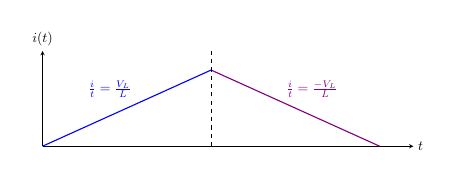
\begin{tikzpicture}
        [
            scale = 0.5,
            >=latex
        ]
        \begin{axis}
            [
                width=11cm,
                height=4cm,
                xmin=0, xmax=11, ymin=0, ymax=5, axis lines=middle,
                x label style={anchor=west},
                xlabel=$t$,
                y label style={anchor=south},
                ylabel=$i(t)$,
                ticks=none
                %grid
            ]
            
            %nodes
            \node                       (m)     at (5,4)        {};
            \node                       (e)     at (10, 0)      {};
            \node[color=blue]           (s1)    at (2, 3)       {$\frac{\diff i}{\diff t} = \frac{V_L}{L}$};
            \node[color=violet]         (s2)    at (8, 3)       {$\frac{\diff i}{\diff t} = \frac{-V_L}{L}$};

            plots
            \addplot[color=blue, thick, domain=0:5]{0.8*x};
            \addplot[color=violet, thick, domain=5:10]{-0.8*x+8};
            \addplot[dashed]coordinates {(5, 0) (5, 5)};
        \end{axis}
        % \node[label={below:\tiny $t = 0$}](t0)    at (0, 0)       {};
    \end{tikzpicture}
\end{center}

\end{minipage}

\begin{tabular}{l | l}
    \textbf{\cbl{1. Phase}} Energie in Spule speichern  & \textbf{\cvt{2. Phase}} Entmagnetisierung \\
    \midrule
    \tabitem Schalter geschlossen                       & \tabitem Schalter offen \\
    \tabitem $V_L = V_{in}$ liegt an Spule an           & \tabitem Strom sinkt, wenn $V_{out} > V_{in}$ \\
    \tabitem $i_L$ muss nicht bei $I_0 = 0$ starten!    & \tabitem Eingeschwungener Zustand: $i_L = I_0$ \\
\end{tabular}

\vspace{0.2cm}
In \textbf{beiden Phasen} gelten die folgenden Formeln:

\renewcommand{\arraystretch}{1.2}
\begin{tabular}{ll}
    \cbl{Ladephase}                 & $ \Delta I_{L_{on}} = \frac{1}{L} \cdot V_{in} \cdot t_{on}$ \\
                                    & $ I_{L_{on}} = \frac{1}{L} \cdot V_{in} \cdot t_{on} + I_0 $\\ 
    \cvt{Entladephase}              & $ \Delta I_{L_{off}} = \frac{1}{L} \cdot (V_{in}- V_{out}) \cdot t_{off}$ \\ 
                                    & $I_{L_{off}} = \frac{1}{L} \cdot (V_{in}- V_{out}) \cdot t_{off} + I_0$ \\
    Gleichgewicht (eingeschwungen)  & $ \Delta I_{L_{on}} = - \Delta I_{L_{off}}$ \\ 
    Ausgangsspannung                & $V_{out} = V_{in} \cdot \Big( 1 + \frac{t_{on}}{t_{off}} \Big)$  \\
\end{tabular}
\renewcommand{\arraystretch}{1}

\vspace{0.2cm}
Die \textbf{Ausgangsspannung} $V_{out}$ ist \textbf{abhängig von der Last} 
\textrightarrow\ Bei hochohmiger Last kann die Ausgangsspannung sehr gross werden!

\subsubsection{Synchronous Boost Converter}

\begin{minipage}{0.4\columnwidth}
    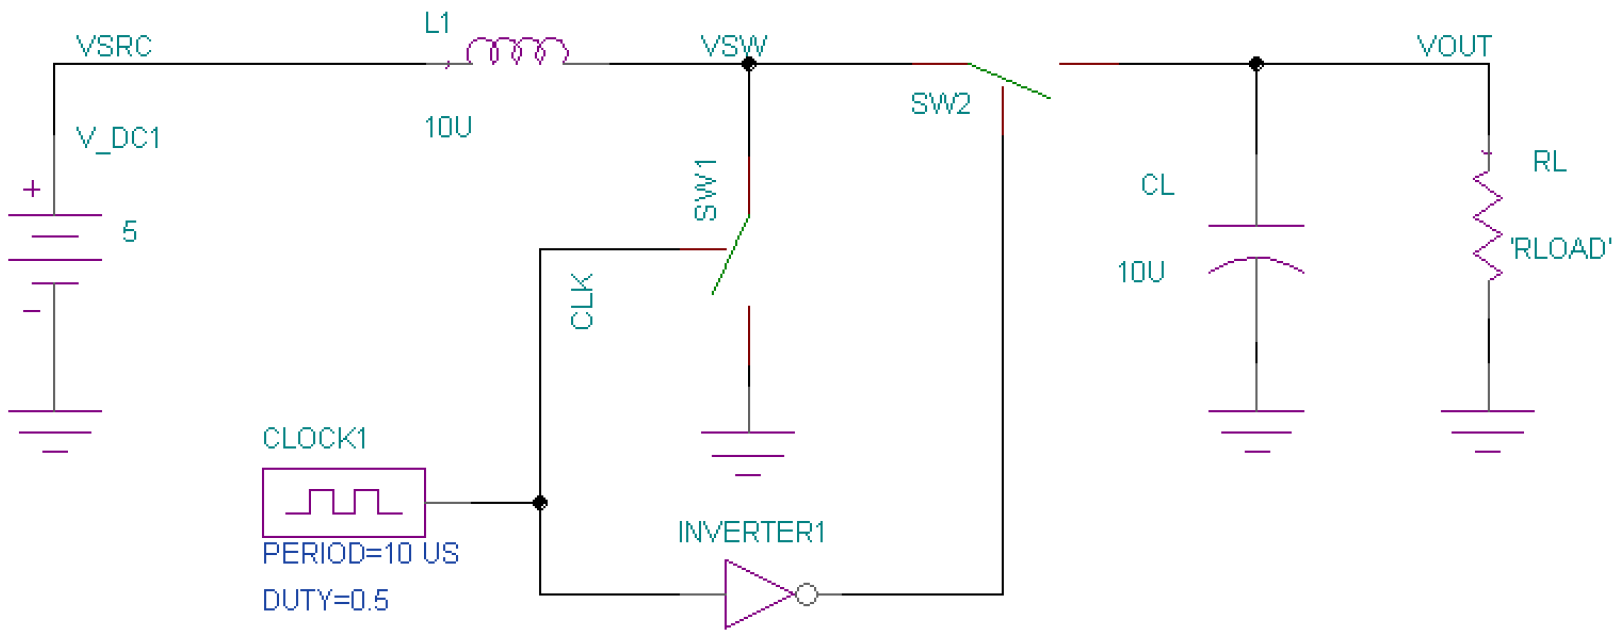
\includegraphics[width=\columnwidth]{images/synchronous_boost_converter.png}
\end{minipage}
\hfill
\begin{minipage}{0.58\columnwidth}
    \begin{itemize}
        \item Diode ersetzt durch Schalter SW2
        \item Entweder SW1 \textbf{oder} SW2 geschlossen
        \item VSW somit immer leitend verbunden, entweder mit GND oder mit $V_{out}$ \\
            \textrightarrow\ In Spule fliesst immer ein Strom
    \end{itemize}
\end{minipage}

\textbf{Achtung:} Bei kleinen Lasten fliesst Strom in die Quelle zurück und die Verlustleistung in der Spule ist grösser (Drahtwiderstand)


\subsection{Aufwärtswandler: Lückender Betrieb}

\begin{minipage}{0.42\columnwidth}
    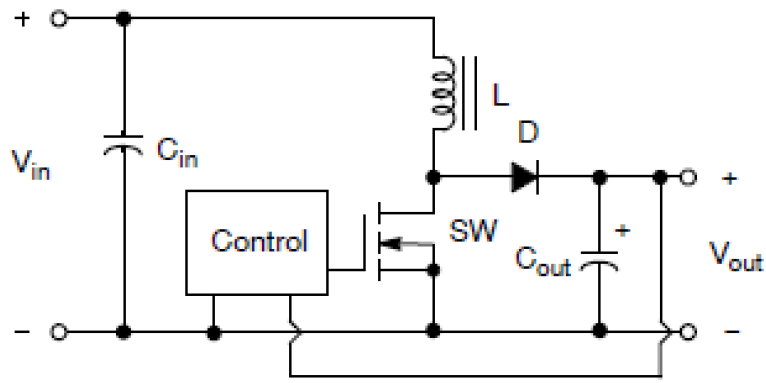
\includegraphics[width=\columnwidth]{images/boost_lueckend.png}
\end{minipage}
\hfill
\begin{minipage}{0.5\columnwidth}
    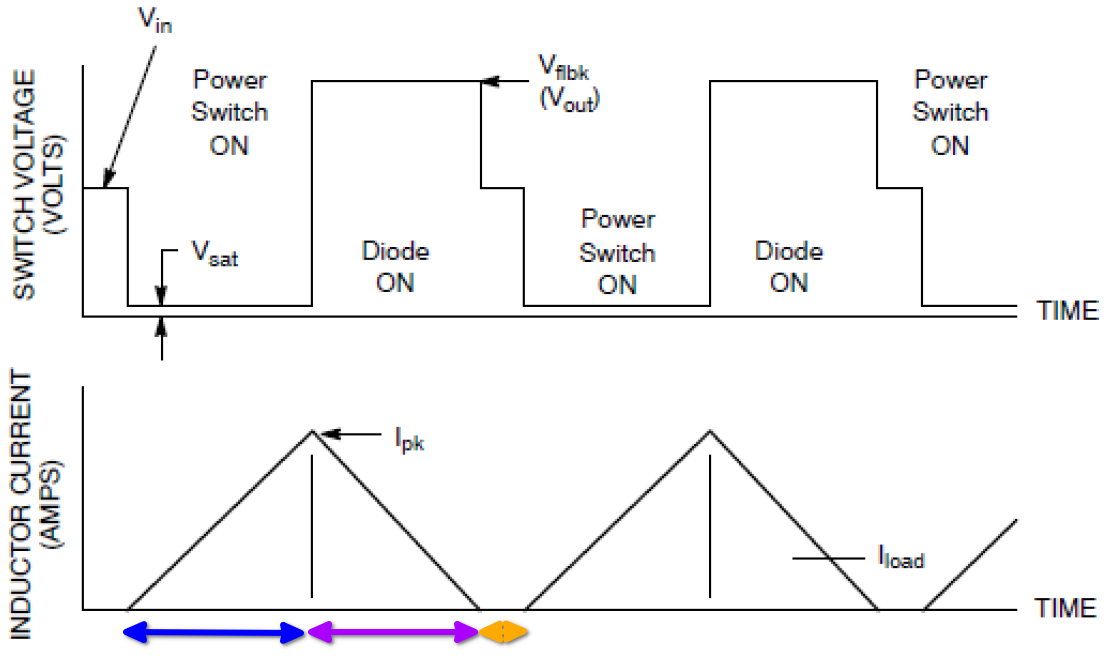
\includegraphics[width=\columnwidth]{images/boost_lueckend_timing.png}
\end{minipage}

\begin{itemize}
    \item Es existiert ein \cor{3. Zustand}, in welchem kein Strom durch Spule fliesst
    \item Aus $i_L = 0$ folgt $V_L = 0$
    \item Schalter SW offen, damit Spannung am Knoten SW $= V_{in}$ wird \textrightarrow\ Diode sperrt
    \item Control schliesst Schalter, nachdem $V_{out} < V_{out,soll}$ ist \textrightarrow\ \textbf{Regelung} von $V_{out}$
\end{itemize}


\subsubsection{Regelung der Ausgangsspannung: voltage-mode control}

\begin{minipage}{0.42\columnwidth}
    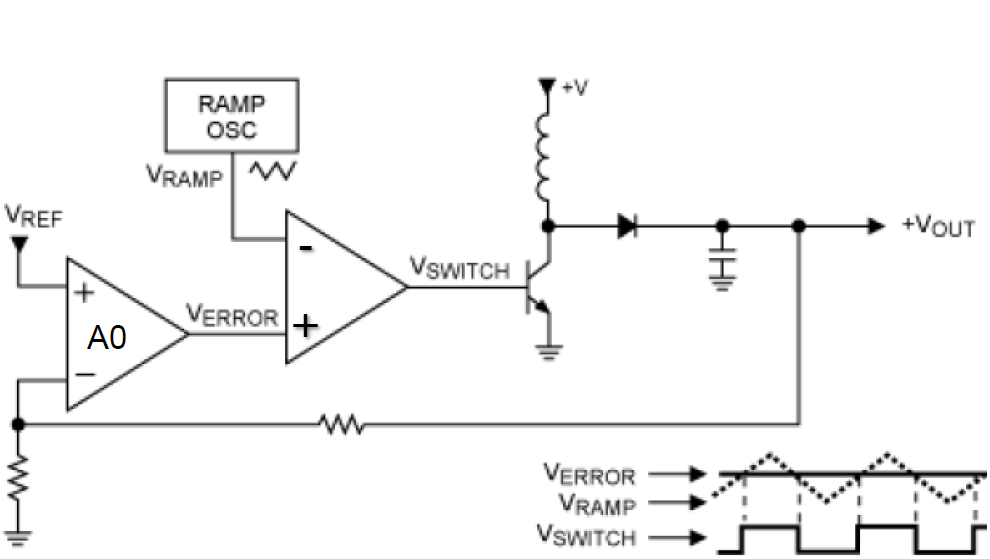
\includegraphics[width=\columnwidth]{images/regelung_ausgangsspannung_voltage.png}
\end{minipage}
\hfill
\begin{minipage}{0.56\columnwidth}
    \begin{itemize}
        \item Verstärker mit Verstäkung A0
        \item Komparator vergleicht $V_{ERROR}$ mit $V_{RAMP}$
        \item $V_{OUT} - V_{REF} \, \Uparrow$,  $V_{ERROR} \Uparrow$, Schalter muss 
            länger geschlossen bleiben \textrightarrow\ grösserer Duty Cycle \textrightarrow\ $V_{OUT} \, \Uparrow$
    \end{itemize}
\end{minipage}


\subsubsection{Regelung der Ausgangsspannung: current-mode control}

\begin{minipage}{0.42\columnwidth}
    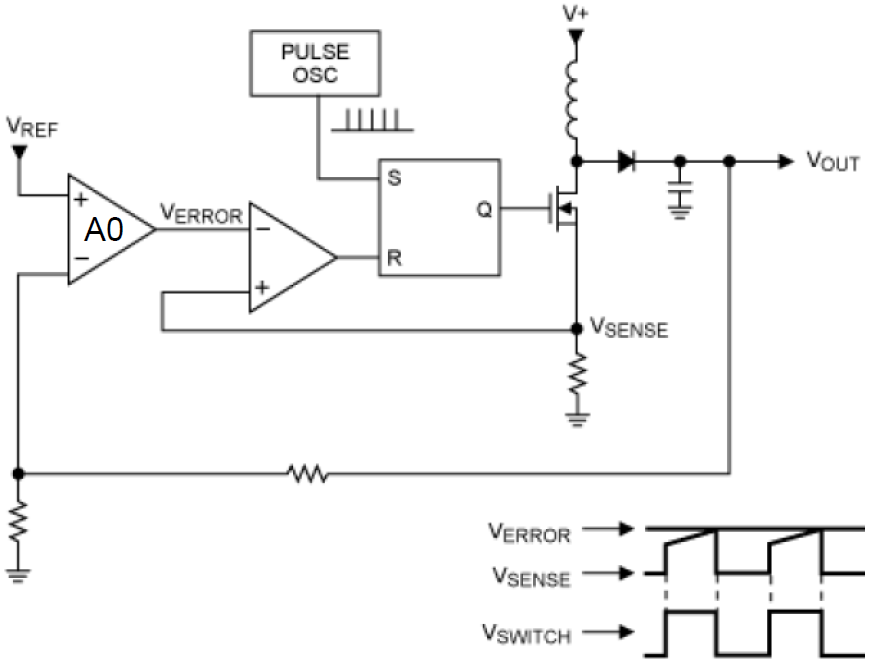
\includegraphics[width=\columnwidth]{images/regelung_ausgangsspannung_current.png}
\end{minipage}
\hfill
\begin{minipage}{0.56\columnwidth}
    \begin{itemize}
        \item Strom wird mit Shund-Widerstand durch Spannung $V_{SENSE}$ gemessen
        \item Verstärker mit Verstäkung A0
        \item Komparator resettiert Flip-Flop \textrightarrow\ Schalter (FET) öffnet
        \item Häufiger zur Regelung verwendet als vorherige Schaltung
    \end{itemize}
\end{minipage}


\subsection{Abwärtswandler (Buck, Step-Down Converter)}

\begin{minipage}[c]{0.4\columnwidth}
    % Abwärtswandler (Buck, Step Down Converter)
% 
% Author:   Alex Krieg
% Date:     02.04.2024

\begin{center}
    \scalebox{0.6}{%
            \begin{circuitikz}[thick]
            % Gitternetzlinien im Hintergrund
            %\draw[xstep=1cm, ystep=1cm, line width=0.1mm, color=lightgray] (0,0) grid (6,4);

            % Einstellungen für Symbole
            \ctikzset
            {  
                inductor            =   american, 
                resistor            =   european,
                inductors/scale     =   1.0, 
                capacitors/scale    =   0.8,
                diodes/scale        =   0.6,
                line width          =   0.5,
            }
            \def\labelOffset{0.4}

            % Knoten
            \coordinate (input) at (0,2);
            \coordinate (K1) at (2,2);
            \coordinate (K2) at (4,2);
            \coordinate (output) at (5,2);
            \coordinate (G1) at (2,0);
            \coordinate (G2) at (4,0);

            % Kreuzungspunkte
            \draw (input)   node[circ]{};
            \draw (K1)      node[circ]{};
            \draw (K2)      node[circ]{};
            \draw (output)  node[circ]{};

            % Knotenbeschriftungen
            \node at ($(input)+(0,\labelOffset)$)  {$V_{IN}$};
            \node at ($(output)+(0,\labelOffset)$) {$V_{OUT}$};

            % Schaltung
            %      Start Pos    Symbol type             Name    End Pos
            \draw (input)   to [normal open switch,     l=$S$]  (K1);               % Schalter
            \draw (K1)      to [L,                      l=$L$]  (K2);               % Suple
            \draw (G1)      to [diode,                  l=$D$]  (K1);               % Diode
            \draw (K2)      to [curved capacitor,       l=$C$]  (G2);               % Kondensator
            \node at ($(G2) + (0.2,1.3)$)  {+};                                     % + Symbol am Kondensator

            \draw (K2)      to [short](output);

            \draw (G1)      node[tlground](GND){}; 
            \draw (G2)      node[tlground](GND){}; 
        \end{circuitikz}
    }
\end{center}
\end{minipage}
\hfill
\begin{minipage}[c]{0.58\columnwidth}
    \begin{center}
    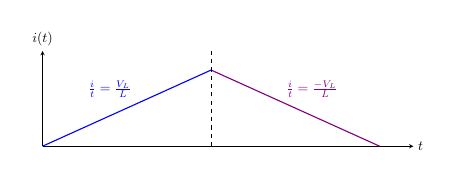
\begin{tikzpicture}
        [
            scale = 0.5,
            >=latex
        ]
        \begin{axis}
            [
                width=11cm,
                height=4cm,
                xmin=0, xmax=11, ymin=0, ymax=5, axis lines=middle,
                x label style={anchor=west},
                xlabel=$t$,
                y label style={anchor=south},
                ylabel=$i(t)$,
                ticks=none
                %grid
            ]
            
            %nodes
            \node                       (m)     at (5,4)        {};
            \node                       (e)     at (10, 0)      {};
            \node[color=blue]           (s1)    at (2, 3)       {$\frac{\diff i}{\diff t} = \frac{V_L}{L}$};
            \node[color=violet]         (s2)    at (8, 3)       {$\frac{\diff i}{\diff t} = \frac{-V_L}{L}$};

            plots
            \addplot[color=blue, thick, domain=0:5]{0.8*x};
            \addplot[color=violet, thick, domain=5:10]{-0.8*x+8};
            \addplot[dashed]coordinates {(5, 0) (5, 5)};
        \end{axis}
        % \node[label={below:\tiny $t = 0$}](t0)    at (0, 0)       {};
    \end{tikzpicture}
\end{center}

\end{minipage}

\vspace{0.2cm}
\textbf{Vereinfachungen:} $V_{out}$ konstant, kein Spannungsabfall über Diode und Schalter \\
\textbf{Formeln gelten nur, wenn immer ein Strom in der Spule fliesst}
\vspace{0.2cm}

\renewcommand{\arraystretch}{1.2}
\begin{tabular}{ll}
    \cbl{Ladephase}                 & $ \Delta I_{L_{on}} = \frac{1}{L} \cdot (V_{in}- V_{out}) \cdot t_{on}$ \\
                                    & $ I_{L_{on}} = \frac{1}{L} \cdot (V_{in}- V_{out}) \cdot t_{on} + I_0 $\\ 
    \cvt{Entladephase}              & $ \Delta I_{L_{off}} = - \frac{1}{L} \cdot V_{out} \cdot t_{off}$ \\ 
                                    & $I_{L_{off}} = - \frac{1}{L} \cdot V_{out} \cdot t_{off} + I_0$ \\
    Gleichgewicht (eingeschwungen)  & $ \Delta I_{L_{on}} = - \Delta I_{L_{off}}$ \\ 
    Ausgangsspannung                & $V_{out} = V_{in} \cdot \frac{t_{on}}{T}$
\end{tabular}
\renewcommand{\arraystretch}{1}


\subsection{Invertierender Wandler (Buck-Boost Converter)}

\begin{minipage}[c]{0.4\columnwidth}
    % Inverting (Invertierender Wandler)
% 
% Author:   Alex Krieg
% Date:     02.04.2024


\begin{center}
    \scalebox{0.6}{%
        \begin{circuitikz}[thick]
            % Gitternetzlinien im Hintergrund
            %\draw[xstep=1cm, ystep=1cm, line width=0.1mm, color=lightgray] (0,0) grid (6,4);

            % Einstellungen für Symbole
            \ctikzset
            {  
                inductor            =   american, 
                resistor            =   european,
                inductors/scale     =   1.0, 
                capacitors/scale    =   0.8,
                diodes/scale        =   0.6,
                line width          =   0.5,
            }
            \def\labelOffset{0.4}

            % Knoten
            \coordinate (input) at (0,2);
            \coordinate (K1) at (2,2);
            \coordinate (K2) at (4,2);
            \coordinate (output) at (5,2);
            \coordinate (G1) at (2,0);
            \coordinate (G2) at (4,0);

            % Kreuzungspunkte
            \draw (input)   node[circ]{};
            \draw (K1)      node[circ]{};
            \draw (K2)      node[circ]{};
            \draw (output)  node[circ]{};

            % Knotenbeschriftungen
            \node at ($(input)+(0,\labelOffset)$)  {$V_{IN}$};
            \node at ($(output)+(0,\labelOffset)$) {$V_{OUT}$};

            % Schaltung
            %      Start Pos    Symbol type             Name    End Pos
            \draw (input)   to [normal open switch,     l=$S$]  (K1);               % Schalter
            \draw (K1)      to [L,                      l=$L$]  (G1);               % Suple
            \draw (K2)      to [diode,                  l=$D$]  (K1);               % Diode
            \draw (G2)      to [curved capacitor,       l=$C$]  (K2);               % Kondensator
            \node at ($(G2) + (0.2,0.7)$)  {+};                                     % + Symbol am Kondensator

            \draw (K2)      to [short](output);

            \draw (G1)      node[tlground](GND){}; 
            \draw (G2)      node[tlground](GND){}; 
        \end{circuitikz}
    }
\end{center}


\end{minipage}
\hfill
\begin{minipage}[c]{0.46\columnwidth}
    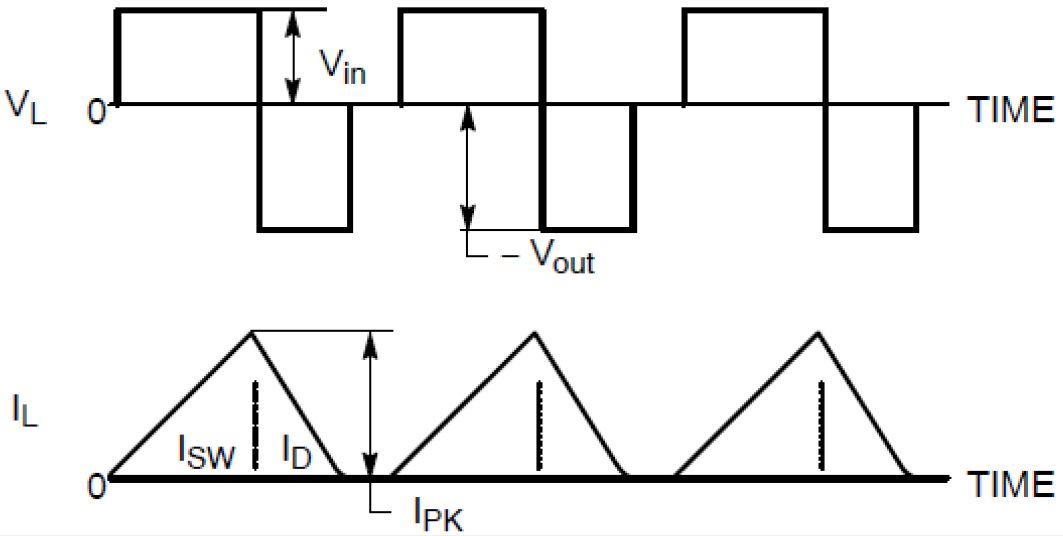
\includegraphics[width=\columnwidth]{images/buck_boost_timing.png}
\end{minipage}

\textbf{Der Converter kann im buck-mode oder boost-mode betrieben werden}
buck-mode: Duty Cycle $\frac{t_{on}}{T} < 0.5$ ; boost-mode: Duty Cycle $\frac{t_{on}}{T} > 0.5$ 

\begin{tabular}{ll}
    \cbl{Ladephase}                     & $ \Delta I_{L_{on}} = \frac{1}{L} \cdot V_{in} \cdot t_{on}$ \\
    \cvt{Entladephase} ($V_{out} < 0$)  & $ \Delta I_{L_{off}} = \frac{1}{L} \cdot V_{out} \cdot t_{off}$ \\ 
    Gleichgewicht (eingeschwungen)      & $ \Delta I_{L_{on}} = - \Delta I_{L_{off}}$ \\ 
    Ausgangsspannung                    & $V_{out} = - V_{in} \cdot \frac{t_{on}}{t_{off}}$  \\
\end{tabular}
\renewcommand{\arraystretch}{1}


\subsection{Flyback (Sperrwandler)}

\begin{minipage}[c]{0.4\columnwidth}
    \begin{center}
    \scalebox{0.5}{%
        \begin{circuitikz}[thick]
            %\draw[xstep=1cm, ystep=1cm, line width=0.1mm, color=lightgray] (0,0) grid (10cm,10cm);

            % Einstellungen für Symbole
            \ctikzset{
                inductor            =   american,
                inductors/scale     =   1.0,
                capacitors/scale    =   0.8,
                diodes/scale        =   0.6,
                line width          =   0.5,
            }
            \def\labelOffset{0.4}

            % Knoten
            \coordinate (input) at (0,3);
            \coordinate (P1) at (0,1);
            \coordinate (K1) at (6,3);
            \coordinate (K2) at (6,1);
            \coordinate (G) at (0,0.5);
            \coordinate (output1) at ($(K1) + (1,0)$);
            \coordinate (output2) at ($(K2) + (1,0)$);

            % Kreuzungspunkte
            \draw (input)   node[circ]{};
            \draw (K1)      node[circ]{};
            \draw (K2)      node[circ]{};
            \draw (output1)      node[circ]{};
            \draw (output2)      node[circ]{};

            % Knotenbeschriftungen
            \node at ($(input)+(0,\labelOffset)$)  {$V_{IN}$};
            \node at ($(output1)+(0,\labelOffset)$) {$V_{OUT}$};

            %Trafo%
            \draw (3,2) node[transformer, scale=0.95] (T) {}
            (T.A1) node[anchor=east] {} %A1
            (T.A2) node[anchor=east] {} %A2
            (T.B1) node[anchor=west] {} %B1
            (T.B2) node[anchor=west] {} %B2
            (T.base) node{T}
            (T.inner dot A2) node[circ]{}
            (T.inner dot B1) node[circ]{};

            %      Start Pos    Symbol type             Name        End Pos
            \draw (G)         node[tlground                    ]  {};             % GND
            \draw (0,1)         to [normal open switch,     l=$S$]  (T.A2) {};      % Switch
            \draw (T.B1)        to [diode,                  l=$D$]  (K1);          % Diode
            \draw (K1)          to [curved capacitor,       l=$C$]  (K2);           % Kondensator
            \node at ($(K2) + (0.2,1.3)$)  {+};                                     % + Symbol am Kondensator

            % Verbindungen
            \draw (input) [short] (T.A1);
            \draw (G) |- (0.1,1);
            \draw (input) -- (T.A1);
            \draw (T.B2) -- (output2);
            \draw (K1) -- (output1);

        \end{circuitikz}
    }
\end{center}


\end{minipage}
\hfill
\begin{minipage}[c]{0.58\columnwidth}
    \begin{itemize}
        \item Ermöglicht \textbf{galvanische Trennung} zwischen Ein- und Ausgang
        \item Transformator mit grosser Induktivität nötig zur Energiespeicherung (mit Luftspalt)
    \end{itemize}
\end{minipage}


\begin{outline}
    \1 Phase 1 (Schalter geschlossen)
        \2 Linear steigender Strom auf Primärseite; Energie wird im Magnetfeld gespeichert
    \1 Phase 2 (Schalter offen)
        \2 Linear sinkender Strom auf Sekundärseite; Magnetfeld baut sich über Sekundärspule ab
    \1 Phase 3 (LC-Schwingkreis)
        \2C parallel zu Schalter auf Primärseite wird wirksam 
\end{outline}


\subsection{Power Fail Control (PFC)}

\begin{minipage}[c]{0.42\columnwidth}
    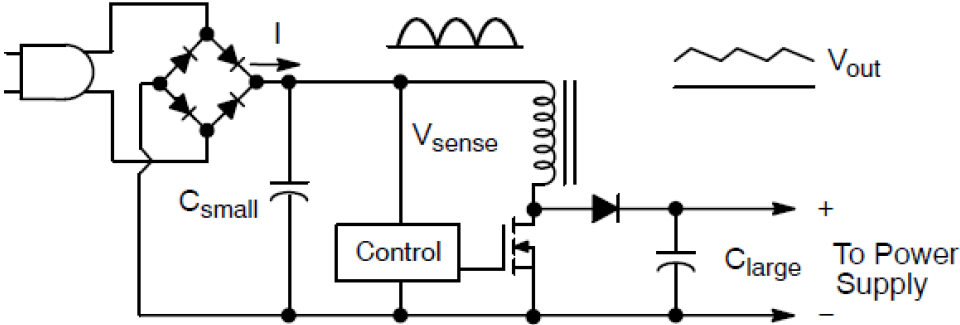
\includegraphics[width=\columnwidth]{images/pfc_schaltung.png}
\end{minipage}
\hfill
\begin{minipage}[c]{0.42\columnwidth}
    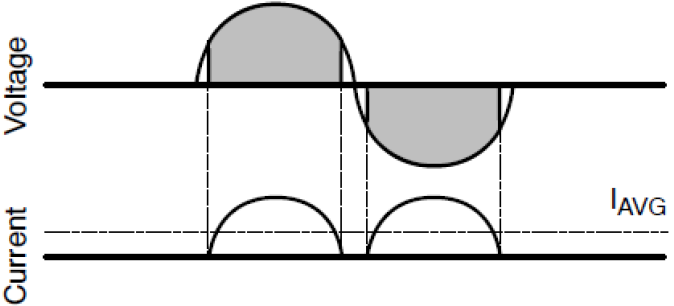
\includegraphics[width=\columnwidth]{images/pfc.png}
\end{minipage}

\begin{minipage}[c]{0.48\columnwidth}
    \begin{center}
        \myul{Ohne PFC}
    \end{center}
    \begin{itemize}
        \item Strom fliesst nur wenn $V_{in} > V_C$\\
            (nur bei Spannungsmaximum) \\
            \textrightarrow\ erzeugt Oberwellen (Blindleistung)
    \end{itemize}
\end{minipage}
\hfill
\begin{minipage}[c]{0.48\columnwidth}
    \begin{center}
        \myul{Mit PFC}
    \end{center}
    \begin{itemize}
        \item Strom soll \textbf{möglichst sinusförmig} fliessen, nicht nur beim Spannungsmaximum
        \item Lösung: 1. Stufe mit Boost Converter
    \end{itemize}
\end{minipage}


\subsection{Aufbau Modernes Netzteil}

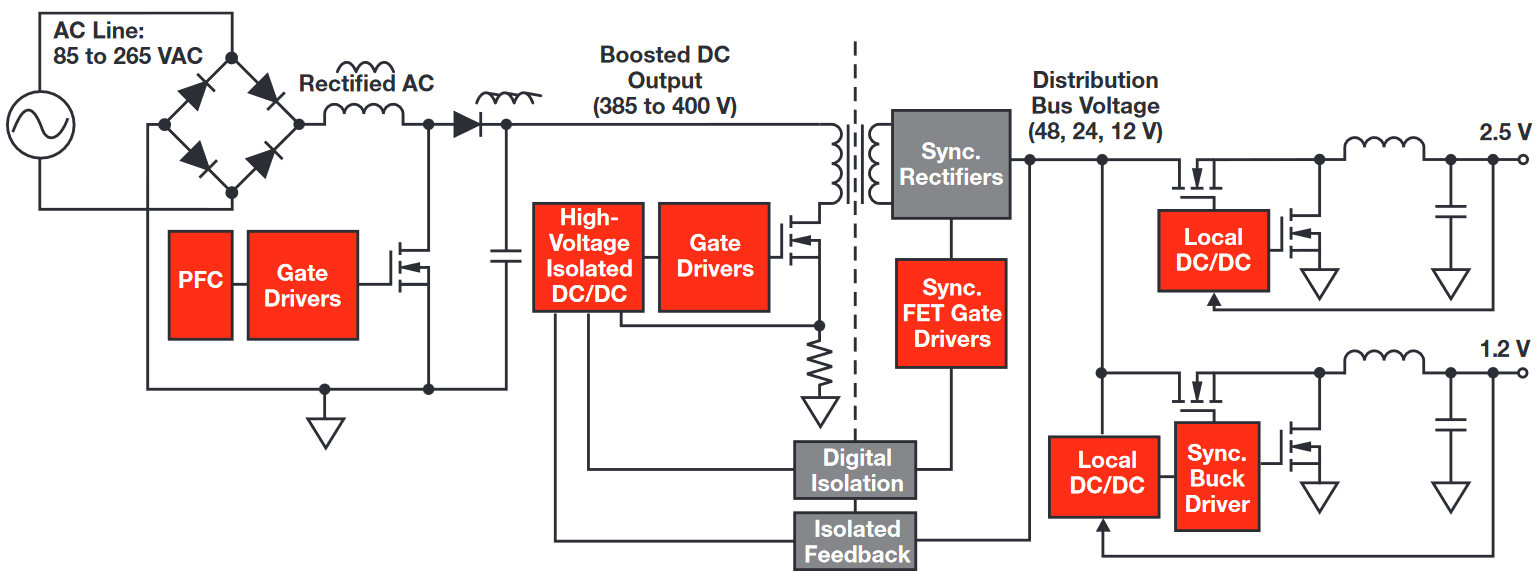
\includegraphics[width=\columnwidth]{images/modernes_netzteil.png}

\begin{itemize}
    \item 1. Stufe: Gleichrichtung und Boost Converter mit PFC
    \item 2. Stufe: Reduktion auf Systemspannung (Bus voltage) mit Flyback-Converter
    \item 3. Stufe: Buck Converter (ev. mehrere)
\end{itemize}


\subsection{Fazit Spannungswandler SMPS}

\begin{itemize}
    \item Geschaltete Spannungsregler generrieren weniger Verlustleistung als Linearregler
    \item Ausgangsspannung geschalteter Spannungsregler hat \textbf{Rippel} der Schaltfrequenz \\
        \textrightarrow\ Muss ev. mit Linearrregler zusätzlich stabilisiert werden
\end{itemize}